\usetikzlibrary{decorations.pathreplacing}

\section*{(11\textordfeminine\ aula) --- Os Postulados da Mecânica Quântica (Seções 4.1 e 4.2)}

Após a introdução à matemática dos espaços vetoriais, estamos prontos para começar a discutir a Mecânica Quântica.

Como vimos na aula anterior, a descrição da dinâmica de elétrons, prótons, átomos etc. deve ser feita de uma maneira diferente da usada para descrever o movimento de satélites, bolas de gude, piões etc.

Assim como no curso de Mecânica Clássica você aprendeu a descrever o movimento de objetos macroscópicos sob influência de forças externas (resolvendo $F=ma$ ou as equações de Lagrange), aqui você irá descrever o movimento de partículas MICROSCÓPICAS\footnote{Note que aquelas que são inevitavelmente perturbadas pela medida.} sob influência de forças.

Considere os 4 ``postulados'' abaixo, usados na Mecânica Clássica e na Mecânica Quântica para descrever uma partícula que se move em 1D sob a influência de forças (conservativas).

\subsection*{Postulado I}

\fbox{\parbox{0.92\textwidth}{
\textbf{MECÂNICA CLÁSSICA:} O estado da partícula em qualquer tempo é especificado por $x(t)$ e $p(t)$.

\textbf{MECÂNICA QUÂNTICA:} O estado da partícula é especificado por um vetor $\ket{\psi(t)}$ no espaço vetorial das funções complexas em 1D.
}}

\begin{quote}
\textbf{Observação:} Veja a diferença: passamos de 2 funções do tempo para um vetor abstrato que evolui no tempo (daí a necessidade de se saber bem a matemática dos ESPAÇOS VETORIAIS).
\end{quote}

\subsection*{Postulado II}

\fbox{\parbox{0.92\textwidth}{
\textbf{MECÂNICA CLÁSSICA:} Toda variável dinâmica é uma função de $x$ e $p$: $\omega = \omega(x,p)$.

\textbf{MECÂNICA QUÂNTICA:} As variáveis $x$ e $p$ da Mecânica Clássica são representadas por OPERADORES HERMITIANOS $\hat{X}$ e $\hat{P} = \hbar \hat{K}$ (definidos na seção 1.10). O operador hermitiano associado a uma outra variável dinâmica é obtido da expressão clássica:
\begin{equation}
\hat{\Omega} = \omega(x \rightarrow \hat{X},\ p \rightarrow \hat{P})
\end{equation}
}}

\begin{quote}
\textbf{Observação:} O operador momentum linear é $\hat{P} = \hbar \hat{K}$, onde $\hbar = \dfrac{h}{2\pi}$ e $\hat{K}$ é o operador definido na seção 1.10.
\end{quote}

\begin{quote}
\textbf{Observação:} ``Variável dinâmica'' pode ser o momento angular, a Hamiltoniana, o momento linear, a posição, a velocidade; QUALQUER COISA QUE POSSA SER ESCRITA EM FUNÇÃO DE $x$ E $p$.
\end{quote}

\begin{quote}
\textbf{Observação:} Como exemplo, a função Hamiltoniana do oscilador harmônico é
\begin{equation}
H(x,p) = \frac{p^2}{2m} + \frac{1}{2}m\omega^2 x^2,
\end{equation}
o operador correspondente na Mecânica Quântica é
\begin{equation}
\hat{H} = \frac{\hat{P}^2}{2m} + \frac{1}{2}m\omega^2 \hat{X}^2.
\end{equation}
\end{quote}

\subsection*{Postulado III}

\fbox{\parbox{0.92\textwidth}{
\textbf{MECÂNICA CLÁSSICA:} Se a partícula está no estado $(x,p)$, a medida da variável $\omega$ resultará em $\omega(x,p)$. O estado da partícula NÃO é alterado pela medida.

\textbf{MECÂNICA QUÂNTICA:} Se a partícula está no estado $\ket{\psi}$, a medida de $\hat{\Omega}$ resultará em um dos AUTOVALORES do operador $\hat{\Omega}$. A PROBABILIDADE de se obter um dos autovalores na medida é proporcional a $\left|\hat{P}_{\omega_i}\ket{\psi}\right|^2$ (a norma ao quadrado da PROJEÇÃO de $\ket{\psi}$ no subespaço do autovalor $\omega_i$), onde $\hat{P}_{\omega_i}$ é o PROJETOR no subespaço do autovalor $\omega_i$. Após a medida que produziu $\omega_i$ como resultado, o estado da partícula passa a ser $\hat{P}_{\omega_i}\ket{\psi}$ (esse é o colapso do vetor de estado).
}}

\begin{quote}
\textbf{Observação:} Em ambos os casos (tanto na Mecânica Clássica quanto na Mecânica Quântica) a ``medida de $\omega$'' se refere a uma MEDIDA IDEAL (a ser definida mais adiante). A Mecânica Quântica diz que, mesmo uma medida ideal perturba o estado de elétrons, prótons, etc.
\end{quote}

\begin{quote}
\textbf{Observação:} O postulado III da Mecânica Quântica diz exatamente como uma medida ideal perturba o estado da partícula.
\end{quote}

\begin{quote}
\textbf{Observação:} O postulado III diz que, conhecendo $\ket{\psi}$, só podemos saber a PROBABILIDADE do resultado da medida de $\hat{\Omega}$ resultar em $\omega_i$ (um dos autovalores).
\end{quote}

Imagine que o operador $\hat{\Omega}$ tenha 3 autovalores $\{\omega_1, \omega_2, \omega_3\}$. Uma série de medidas de $\hat{\Omega}$ no mesmo estado $\ket{\psi}$ resultaria em algo como o diagrama abaixo, onde cada medida individual produz um dos três autovalores, de forma aparentemente aleatória, em função do número da medida:

\begin{center}
\begin{tabular}{c}
$\omega_3$ : $\times$\quad\ \ $\times\ \times\ \times\ \ \ \times$\\
$\omega_2$ : \ \ \ \ $\times$\ \ \quad\quad\ \ \ \ \ $\times\ \times$\\
$\omega_1$ : \ \ \quad\quad$\times\ \times$\\
\qquad\ \ 1\ \ 2\ \ 3\ \ 4\ \ 5\ \ 6\ \ 7\ \ 8 \ \ \ldots\ (\# da medida)
\end{tabular}
\end{center}

NÃO HÁ COMO PREVER O RESULTADO DE UMA MEDIDA EM PARTICULAR, apenas podemos prever a DISTRIBUIÇÃO dos resultados de UMA SÉRIE DE MEDIDAS.

Lembre dos fótons ou elétrons formando as franjas de interferência do experimento de fenda dupla. Lá também é impossível prever onde um determinado fóton ou elétron irá aparecer, apenas é mais provável que ele apareça num máximo da figura de interferência do que em um mínimo.

No caso da variável $\hat{\Omega}$ acima, se $\left|\hat{P}_{\omega_3}\ket{\psi}\right|^2 > \left|\hat{P}_{\omega_1}\ket{\psi}\right|^2$, o resultado $\omega_3$ será mais obtido (em uma série de medidas) que o resultado $\omega_1$.

\begin{quote}
\textbf{Observação:} É desse postulado que vem a QUANTIZAÇÃO. As variáveis clássicas $\omega(x,p)$ são funções contínuas que podem assumir qualquer valor real (talvez em algum intervalo limitado), no entanto, o operador associado $\hat{\Omega}$ pode ter um espectro discreto $\{\omega_1, \omega_2, \dots\}$ e, dessa forma, só admitir CERTOS VALORES como resultado da medida de $\hat{\Omega}$.
\end{quote}

\subsection*{Postulado IV}

\fbox{\parbox{0.92\textwidth}{
\textbf{MECÂNICA CLÁSSICA:} As variáveis $x$ e $p$ mudam com o tempo de acordo com
\begin{equation}
\dot{x} = \frac{\partial H}{\partial p}, \qquad \dot{p} = -\frac{\partial H}{\partial x},
\end{equation}
onde $H(x,p)$ é a função Hamiltoniana.

\textbf{MECÂNICA QUÂNTICA:} O estado $\ket{\psi(t)}$ evolui no tempo de acordo com a Equação de Schrödinger
\begin{equation}
i\hbar \frac{d}{dt}\ket{\psi(t)} = \hat{H}\ket{\psi(t)},
\end{equation}
onde $\hat{H}$ é o operador Hamiltoniano obtido de $\hat{H} = H(x \rightarrow \hat{X},\ p \rightarrow \hat{P})$.
}}

\begin{quote}
\textbf{Observação:} Note o papel central desempenhado pela função Hamiltoniana na Mecânica Clássica e pelo operador Hamiltoniano na Mecânica Quântica. Por exemplo, para uma partícula de massa $m$ submetida a um potencial harmônico, usamos:
\begin{align}
H(x,p) &= \frac{p^2}{2m} + \frac{1}{2}m\omega^2 x^2 \qquad \text{nas Eqs. de Hamilton,}\\
\hat{H} &= \frac{\hat{P}^2}{2m} + \frac{1}{2}m\omega^2 \hat{X}^2 \qquad \text{na Eq. de Schrödinger.}
\end{align}
\end{quote}

\subsection*{Discussão dos postulados I, II e III}

\subsubsection*{Postulado I}

O espaço vetorial da Mecânica Quântica é o espaço das funções complexas (em 1D, se a partícula se move em 1D, ou em 3D se ela se move em 3D). Esse espaço contém:

\begin{enumerate}
\item[i)] funções próprias ou normalizáveis
\begin{equation}
\braket{\psi}{\psi} = \int_{-\infty}^{\infty} \psi^*(x)\psi(x)\, dx < \infty;
\end{equation}
\item[ii)] funções impróprias, não normalizáveis, mas que não divergem no infinito.
\end{enumerate}

Os estados físicos (possíveis de serem produzidos em laboratório) são NORMALIZÁVEIS. Os estados impróprios aparecem como autoestados de certos operadores.

A FUNÇÃO DE ONDA é
\begin{equation}
\label{eq:aula11_funcao_onda}
\psi(x,t) = \braket{x}{\psi(t)} \qquad \text{(em 1D)}.
\end{equation}

\subsubsection*{Postulados II e III}

Suponha que o operador $\hat{\Omega}$ associado a uma variável $\omega(x,p)$ foi construído. Pelo postulado II ele deve ser Hermitiano, portanto seus autovetores podem ser ortonormalizados.

\begin{itemize}
\item Vamos encontrar operadores com ESPECTRO DISCRETO (os autovalores vão poder ser associados a números inteiros chamados NÚMEROS QUÂNTICOS)
\begin{equation}
\braket{\omega_i}{\omega_j} = \delta_{ij} \qquad \text{(ortonormalização)}.
\end{equation}
\item Vamos encontrar também operadores com ESPECTRO CONTÍNUO\footnote{São os autovetores associados à parte contínua do espectro que são impróprios.} (os autovalores caem em uma faixa de números reais). Exemplos são os operadores $\hat{X}$ e $\hat{K}$.
\begin{equation}
\braket{\omega}{\omega'} = \delta(\omega - \omega') \qquad \text{(ortonormalização)}.
\end{equation}
\item Vamos encontrar operadores com uma parte do espectro discreta e outra parte contínua (espectros \textbf{mistos}).
\end{itemize}

Com autovetores ortonormalizados construímos os PROJETORES do postulado III.

Se o espectro de $\hat{\Omega}$ é discreto temos
\begin{equation}
\hat{I} = \sum_{i}\sum_{\alpha} \ket{\omega_i,\alpha}\bra{\omega_i,\alpha}, \qquad \hat{P}_{\omega_i} = \sum_{\alpha} \ket{\omega_i,\alpha}\bra{\omega_i,\alpha},
\end{equation}
onde o índice $i$ é o índice do autovalor e o índice $\alpha$ é o índice de eventuais degenerescências, e $\hat{P}_{\omega_i}$ é o projetor associado ao autovalor $\omega_i$.

A probabilidade de obtermos o autovalor $\omega_i$ ao medirmos $\hat{\Omega}$ no estado $\ket{\psi}$ é
\begin{equation}
P(\omega_i) = N \left|\hat{P}_{\omega_i}\ket{\psi}\right|^2 = N\bra{\psi}\hat{P}_{\omega_i}^\dagger \hat{P}_{\omega_i}\ket{\psi} = N\bra{\psi}\hat{P}_{\omega_i}\ket{\psi},
\end{equation}
onde usamos que $\hat{P}_{\omega_i}$ é Hermitiano e idempotente, e $N$ é a constante de proporcionalidade.

A soma das probabilidades associadas a todos os autovalores deve ser igual a 1. Isso determina $N$:
\begin{equation}
1 = \sum_i P(\omega_i) = N \sum_i \bra{\psi}\sum_\alpha \ket{\omega_i,\alpha}\bra{\omega_i,\alpha}\ket{\psi} = N\braket{\psi}{\psi}.
\end{equation}

Finalmente,
\begin{equation}
\label{eq:aula11_prob_discreta}
\boxed{P(\omega_i) = \frac{\bra{\psi}\hat{P}_{\omega_i}\ket{\psi}}{\braket{\psi}{\psi}}}
\end{equation}
é a probabilidade de encontrar $\omega_i$, medindo $\hat{\Omega}$ no estado $\ket{\psi}$.

\begin{quote}
\textbf{Observação:} Se $\hat{P}_{\omega_i}\ket{\psi} = \ket{\psi}$, o resultado da medida de $\hat{\Omega}$ resulta em $\omega_i$ em 100\% das medidas ($\ket{\psi}$ pertence ao subespaço do autovalor $\omega_i$).
\end{quote}

\begin{quote}
\textbf{Observação:} Se
\begin{equation}
\ket{\psi} = \frac{\alpha\ket{\omega_1} + \beta\ket{\omega_2}}{\sqrt{|\alpha|^2 + |\beta|^2}} \qquad \text{(normalizado)},
\end{equation}
a medida de $\hat{\Omega}$ resulta em:
\begin{itemize}
\item $\omega_1$, com probabilidade $\dfrac{|\alpha|^2}{|\alpha|^2 + |\beta|^2}$,
\item $\omega_2$, com probabilidade $\dfrac{|\beta|^2}{|\alpha|^2 + |\beta|^2}$,
\end{itemize}
e nenhum outro autovalor pode ser obtido.
\end{quote}

\begin{quote}
\textbf{Observação:} Quando expandimos $\ket{\psi}$ na base de autovetores de $\hat{\Omega}$, os coeficientes da expansão fornecem diretamente as probabilidades:
\begin{equation}
\ket{\psi} = \sum_i \sum_\alpha \underbrace{\braket{\omega_i,\alpha}{\psi}}_{c_{i,\alpha}} \ket{\omega_i,\alpha} \quad \Longrightarrow \quad P(\omega_i) = \frac{\sum_\alpha |c_{i,\alpha}|^2}{\braket{\psi}{\psi}}.
\end{equation}
\end{quote}

\textbf{Exemplo:} Suponha
\begin{equation}
\ket{\psi} = \frac{1}{2}\ket{\omega_1} + \frac{1}{2}\ket{\omega_2} + \frac{1}{\sqrt{2}}\ket{\omega_3},
\end{equation}
onde $\{\ket{\omega_i}\}$ é uma base ortonormal. Verifique que $\ket{\psi}$ está normalizado:
\begin{equation}
\braket{\psi}{\psi} = \left(\frac{1}{2}\right)^2 + \left(\frac{1}{2}\right)^2 + \left(\frac{1}{\sqrt{2}}\right)^2 = \frac{1}{4} + \frac{1}{4} + \frac{1}{2} = 1.
\end{equation}

Os únicos resultados possíveis de serem obtidos medindo $\hat{\Omega}$ são:
\begin{itemize}
\item $\omega_1$, com prob. $1/4$,
\item $\omega_2$, com prob. $1/4$,
\item $\omega_3$, com prob. $1/2$,
\end{itemize}
($\omega_4, \omega_5$, etc., se existirem, não serão medidos).

\subsection*{Complicações}

\textbf{1) Em algumas situações a receita para se construir o operador $\hat{\Omega}$ é ambígua.}

Se $\omega(x,p) = xp$, devemos usar $\hat{\Omega}_1 = \hat{X}\hat{P}$ ou $\hat{\Omega}_2 = \hat{P}\hat{X}$? Na verdade, nenhum dos dois é Hermitiano:
\begin{equation}
\hat{\Omega}_1^\dagger = \hat{P}^\dagger \hat{X}^\dagger = \hat{P}\hat{X} \neq \hat{\Omega}_1 \qquad \text{(mesmo para } \hat{\Omega}_2\text{)}.
\end{equation}

Usamos a combinação simétrica e Hermitiana:
\begin{equation}
\label{eq:aula11_simetrizacao}
\boxed{\hat{\Omega} = \frac{1}{2}\left(\hat{X}\hat{P} + \hat{P}\hat{X}\right)}
\end{equation}

\textbf{2) O espectro de $\hat{\Omega}$ tem uma parte CONTÍNUA.}

Nesse caso não faz sentido perguntar qual a probabilidade de encontrar o valor $\omega$ (pertencente ao espectro contínuo) em uma medida de $\hat{\Omega}$, simplesmente porque nenhum aparelho de medida será capaz de selecionar um número real específico em uma faixa de valores possíveis.

\begin{center}
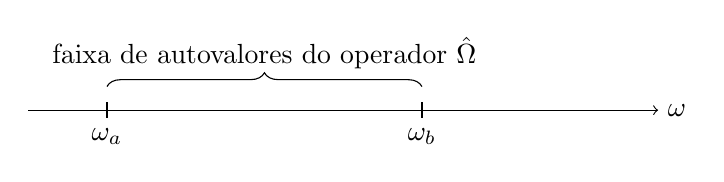
\begin{tikzpicture}
\draw[->] (0,0) -- (8,0) node[right] {$\omega$};
\draw[thick] (1,0.1) -- (1,-0.1) node[below] {$\omega_a$};
\draw[thick] (5,0.1) -- (5,-0.1) node[below] {$\omega_b$};
\draw[decorate,decoration={brace,amplitude=5pt}] (1,0.3) -- (5,0.3) node[midway,above=3pt]{faixa de autovalores do operador $\hat{\Omega}$};
\end{tikzpicture}
\end{center}

Perguntamos qual a probabilidade de, medindo $\hat{\Omega}$, encontrar um resultado em uma FAIXA $[\omega_1,\omega_2]$ dentro do espectro contínuo.

Exatamente como no caso do espectro discreto, a probabilidade é obtida de um projetor:
\begin{equation}
\hat{P}_{[\omega_1,\omega_2]} = \int_{\omega_1}^{\omega_2} \ket{\omega}\bra{\omega}\, d\omega,
\end{equation}
que projeta um estado no subespaço gerado pelos autovetores de $\hat{\Omega}$ com autovalor entre $\omega_1$ e $\omega_2$.

\begin{quote}
\textbf{Observação:} Estou supondo que os autovetores de $\hat{\Omega}$ estão normalizados no sentido da função delta de Dirac, $\braket{\omega}{\omega'} = \delta(\omega-\omega')$.
\end{quote}

\begin{equation}
\label{eq:aula11_prob_continua}
\boxed{P([\omega_1,\omega_2]) = \frac{\left|\hat{P}_{[\omega_1,\omega_2]}\ket{\psi}\right|^2}{\braket{\psi}{\psi}} = \frac{\displaystyle\int_{\omega_1}^{\omega_2} \braket{\psi}{\omega}\braket{\omega}{\psi}\, d\omega}{\braket{\psi}{\psi}}}
\end{equation}

Caso $\braket{\psi}{\psi} = 1$, interpretamos $|\braket{\omega}{\psi}|^2$ como DENSIDADE DE PROBABILIDADE, com dimensão de $[\omega]^{-1}$.

\begin{quote}
\textbf{Observação:} Apenas quando os autovetores impróprios estão normalizados no sentido da função delta de Dirac os projetores se escrevem como $\displaystyle\int d\omega\, \ket{\omega}\bra{\omega}$.
\end{quote}

A probabilidade de obter QUALQUER RESULTADO POSSÍVEL deve ser 1. De fato (admitindo $\braket{\psi}{\psi}=1$):
\begin{align}
P([\omega_a,\omega_b]) &= \underbrace{\int_{\omega_a}^{\omega_b} d\omega\, |\braket{\omega}{\psi}|^2}_{\text{integral sobre todos os valores possíveis de }\omega \text{ (conjunto completo dos autovalores de }\hat{\Omega}\text{)}}\\
&= \int_{\omega_a}^{\omega_b} d\omega\, \braket{\psi}{\omega}\braket{\omega}{\psi}\\
&= \bra{\psi}\hat{I}\ket{\psi} = 1.
\end{align}

\begin{quote}
\textbf{Observação:} Aqui usei $\hat{I} = \displaystyle\int_{\omega_a}^{\omega_b} d\omega\, \ket{\omega}\bra{\omega}$, válida se $\braket{\omega}{\omega'} = \delta(\omega-\omega')$.
\end{quote}

\textbf{Exemplo:} Qual a probabilidade de encontrar o elétron, no estado (normalizado) $\ket{\psi}$, entre $x=a$ e $x=b$?

\begin{equation}
P([a,b]) = \int_a^b dx\, |\braket{x}{\psi}|^2 = \int_a^b dx\, |\psi(x)|^2,
\end{equation}
onde $\ket{x}$ são os autovetores do operador $\hat{X}$ associados à faixa de autovalores da medida, e $|\psi(x)|^2$ é o quadrado da função de onda.

\textbf{3)} Veremos o exemplo de um operador, o spin, que não tem uma variável clássica associada. Nesse caso o experimento irá nos dizer como construir o operador quântico.

\subsection*{Colapso do vetor de estado}

O postulado III diz que, após medir $\hat{\Omega}$ e encontrar o resultado $\omega_i$ (no caso discreto), ou um resultado na faixa $[\omega_1,\omega_2]$ (no caso contínuo), o vetor de estado da partícula passa a ser a projeção de $\ket{\psi}$ no subespaço associado ao resultado da medida\footnote{Salvo pela necessária renormalização do vetor de estado.}:

\begin{align}
\hat{P}_{\omega_i}\ket{\psi} &= \sum_\alpha \ket{\omega_i,\alpha}\braket{\omega_i,\alpha}{\psi} \qquad \text{(caso discreto)}\\
\hat{P}_{[\omega_1,\omega_2]}\ket{\psi} &= \int_{\omega_1}^{\omega_2} d\omega\, \ket{\omega}\braket{\omega}{\psi} \qquad \text{(caso contínuo)}
\end{align}

As ``medidas'' a que se referem os postulados são medidas idealmente precisas e não perturbadoras do estado do sistema. Na prática elas quase sempre envolvem a interação com a radiação eletromagnética.

\subsection*{Medida ideal de momentum}

\begin{center}
\begin{tikzpicture}[>=Stealth]
\node at (-2.7,0.6) {\footnotesize partícula de momentum};
\node at (-2.7,0.3) {\footnotesize bem definido};
\draw[->] (-2,0) -- (-0.8,0) node[midway,above] {$p$};
\filldraw (-0.8,0) circle (1pt);
\draw[->] (-0.8,0) -- (0.5,0.6) node[midway,above] {$\omega$};
\node[above] at (0,0.6) {fóton};
\draw[->] (-0.8,0) -- (2.5,0);
\node[right] at (2.5,0) {$\times$};
\node[below right] at (2.5,0) {(ANTES)};
\node[below] at (0,0) {fóton};

\draw[->] (-2,-1.4) -- (-0.5,-1.4) node[midway,above] {$p'$};
\filldraw (-0.8,-1.4) circle (0pt);
\draw[->] (-0.8,-1.4) -- (1.8,-0.9) node[midway,above] {$\omega'$};
\node[right] at (1.8,-0.9) {(DEPOIS)};
\end{tikzpicture}
\end{center}

Para esse espalhamento Compton ser uma medida ideal de momentum, ele não pode alterar o momentum da partícula, pois, de acordo com o postulado, se a partícula tem um momentum bem definido (está no estado $\ket{\psi} = \ket{p}$)\footnote{Na verdade, uma faixa estreita em torno de $p$, pois o operador $\hat{P} = \hbar\hat{K}$ tem espectro contínuo.}, uma medida de momentum só pode resultar em $p$ e o estado do sistema NÃO IRÁ SE ALTERAR (pois já é um dos autovetores do operador $\hat{P}$).

O momentum do fóton é $\dfrac{\hbar\omega}{c}$ (sua energia $\div\, c$):
\begin{align}
p - \frac{\hbar\omega}{c} &= p' + \frac{\hbar\omega'}{c} \qquad \text{(cons. momentum)}\\
\underbrace{\sqrt{p^2c^2 + m^2c^4}}_{\text{energia inicial da partícula (relativística)}} + \hbar\omega &= \sqrt{p'^2c^2 + m^2c^4} + \hbar\omega' \qquad \text{(cons. energia)}
\end{align}

Aqui você mede $\omega$ e $\omega'$ e, dessas equações, obtém $p$ e $p'$.

Uma medida ideal deve usar um fóton de frequência $\omega$ que permita $p \approx p'$ (i.e., que não altere o valor de $p$, mas que ainda permita determiná-lo).

É fácil ver que se $\omega \to 0$, $p' \to p$ (momentum da partícula não é alterado). Isso seria uma medida ideal de momentum.

\fbox{\parbox{0.92\textwidth}{
UMA MEDIDA IDEAL É AQUELA QUE NÃO ALTERA O ESTADO DO SISTEMA QUANDO ESSE ESTADO É UM DOS AUTOVETORES DO OPERADOR $\hat{\Omega}$.
}}

Uma medida ideal de posição no estado $\ket{p}$ (autovetor do operador $\hat{P}$) altera o estado, pois $\ket{p}$ não é autoestado do operador $\hat{X}$.

Isso é o que o postulado III diz, mas por que deve ser assim? Porque uma medida ideal de posição usa fótons de momentum arbitrariamente grande\footnote{Correspondentes a uma radiação com comprimento de onda muito pequeno.} e que alteram completamente um estado como $\ket{p}$ (mas não alterariam um estado de posição definida como $\ket{x}$).

\fbox{\parbox{0.92\textwidth}{
UMA MEDIDA IDEAL DE $\hat{\Omega}$ DEIXA APENAS OS AUTOVETORES DO OPERADOR $\hat{\Omega}$ INALTERADOS. OUTROS VETORES SÃO ALTERADOS.
}}

``Medida'', no nosso curso, será sempre ``medida ideal'' no sentido acima.

``Medida Ideal'' para a Mecânica Clássica deixa QUALQUER estado $(x,p)$ inalterado, pois para objetos clássicos é possível encontrar uma radiação eletromagnética que permite determinar a posição e o momentum da partícula sem alterar nenhum dos dois (para átomos, elétrons, etc. isso não é possível).
